\documentclass[10pt, a4paper, titlepage]{jsreport}

\usepackage[dvipdfmx]{graphicx}
\usepackage[dvipdfmx]{hyperref}
\usepackage{pxjahyper}
\usepackage{amsmath}
\usepackage{mathtools}
\usepackage{empheq}
\usepackage{listings}

\lstset{
  basicstyle={\ttfamily},
  identifierstyle={\small},
  commentstyle={\smallitshape},
  keywordstyle={\small\bfseries},
  ndkeywordstyle={\small},
  stringstyle={\small\ttfamily},
  frame={tb},
  breaklines=true,
  columns=[l]{fullflexible},
  numbers=left,
  xrightmargin=0zw,
  xleftmargin=3zw,
  numberstyle={\scriptsize},
  stepnumber=1,
  numbersep=1zw,
  lineskip=-0.5ex
}

\title{令和2年度 卒業研究 論文 \\ 秘密分散の実装における速度・容量性能の評価}
\author{三浦夢生}
\date{2021年2月}

\begin{document}
	\maketitle

	\begin{abstract}
		様々なシステムやサービスがディジタル・オンライン化される流れにある現代社会において,情報の紛失や盗難への対策は重要性を増すばかりである.

		これに対する技術として「秘密分散」があげられる.
		%
		秘密分散とは元の秘密情報をアルゴリズムに基づいて作成した分散情報を管理する者や端末に配布・保管し,必要な数だけ集めて復元する技術のことである.

		本研究では秘密分散技術のうち,加法的秘密分散・$(k,n)$しきい値秘密分散・$(k,L,n)$しきい値秘密分散を,シェルスクリプト及びPythonを用いて実装し,秘密分散における一連の処理にかかった時間と生成されたシェアの平均サイズをまとめ,結果をもとに各アルゴリズムについて評価・考察を行う.
	\end{abstract}

	\tableofcontents
	\clearpage

	\chapter{はじめに}
	様々なシステムやサービスがディジタル・オンライン化される流れにある現代社会において,情報の紛失や盗難への対策は重要性を増すばかりである.
	%
	例として,機密情報の複数人による管理や各地に配置されたストレージで情報の保管をする場合などがある.
	%
	また,オンライン決済やネットバンキングの普及により管理しなければならない機密情報なども増えている.
	
	これらに対する技術として「秘密分散」があげられる.
	%
	秘密分散とは元の秘密情報をアルゴリズムに基づいて作成した分散情報を管理する者や端末に配布・保管し,必要な数だけ集めて復元する技術のことである.
	%
	このとき,元の秘密情報から分散情報を作成する者・端末のことを「ディーラー」,配布された分散情報を保守・管理する者・端末を「参加者」,一連の処理において扱われる分散情報を「シェア」という.
	%
	アルゴリズムごとに設定された数だけシェアを集めなければ,元の秘密情報を得ることはできない.
	%
	この技術は秘密情報を分散して管理したり,複数人で秘密情報の完全性を担保したりする性質から,クラウドサービスやブロックチェーンと相性が良いため広く用いられている.

	この技術の代表例としてShamirの提案した$(k,n)$しきい値秘密分散\cite{shamir}があげられる.
	%
	これは元の秘密情報から$n$個のシェアを生成し,$k$個のシェアから秘密情報の復元ができるが,$k-1$以下の個数のシェアからは元の情報は全く得られない手法である.

	本研究では,加法的秘密分散\cite{oohara}・$(k,n)$しきい値秘密分散\cite{shamir}・$(k,L,n)$しきい値秘密分散\cite{yamamoto}\cite{multiparty}の,3通りのアルゴリズムを実装し,実行速度及び生成されたシェアの平均サイズについて評価し,いずれが優れたアルゴリズムか,高速化の余地や改善点について考察を行う.

	\chapter{秘密分散}
	本章では,今回実装した秘密分散アルゴリズムの概要について述べる.

	\section{加法的秘密分散\cite{oohara}}
	加法的秘密分散は$n$個のシェアに対して$n$個のシェアからのみ元の情報が復元できるため,$(n,n)$しきい値秘密分散ともいえる.
	%
	生成されるシェアのサイズは,生成する乱数の範囲によって決まる.

	この手法はまず乱数を用いて,シェア$s_{i},i=2,3,{\cdots},n$を以下のように生成する.
	%
	\begin{eqnarray*}
		s_{2}&=&r_{1} \\
		s_{3}&=&r_{2} \\
		&{\vdots}& \\
		s_{n}&=&r_{n-1}
	\end{eqnarray*}

	次に秘密情報$S$を用いて以下のようにシェア$s_{1}$を生成する.
	%
	\begin{eqnarray*}
		s_{1}=S-(s_{2}+s_{3}+{\cdots}+s_{n})
	\end{eqnarray*}

	復元の際には,参加者に配布したシェアを全て集めて足し合わせることで秘密情報$S$を得る.

	上記の計算を素数$p$を標数とする体の上で行う手法もある.
	%
	また用いる演算が加算のみなので,環上で計算を行うこともできる.
	%
	発展させた手法として,シェアを一人に複数個割り当てることで後述の$(k,n)$しきい値秘密分散を実現する手法($(k,n)$複製型秘密分散という)も示されている.\cite{oohara}

	\section{$(k,n)$しきい値秘密分散\cite{shamir}}
	この手法は開発者の名前をとってShamirの秘密分散とも呼ばれる.
	%
	$(k,n)$しきい値秘密分散は$n$個のシェアに対して$k$個のシェアから元の秘密情報が復元できるが,$(k-1)$個以下のシェアからは元の秘密情報に関する情報は全く得られない.
	%
	生成されるシェアは元の秘密情報と同等のサイズとなる.

	この手法は秘密情報$S$を定数項とする,ランダムな係数をもつ$k-1$次多項式を生成する.
	%
	\begin{eqnarray*}
		f(x)=S+a_{1}x+a_{2}x^{2}+{\cdots}+a_{k-1}x^{k-1}
	\end{eqnarray*}

	また参加者に番号$i$を割り振り,$f(i)$を計算し,シェアとして参加者に渡す.
	%
	復元には$k$個のシェア$(i,f(i)),i=1,2,\cdots,k$を持ち寄り,$k$個の式を立てて連立方程式を解くことで秘密情報$S$が求められる.
	%
	ただし,参加者の番号によらず,決められた数を集めればよい.
	%
	\begin{empheq}[left=\empheqlbrace]{align}
		f(1)&=S+a_{1}{\cdot}1+a_{2}{\cdot}1^{2}+{\cdots}+a_{k-1}{\cdot}1^{k-1} \nonumber \\
		f(2)&=S+a_{1}{\cdot}2+a_{2}{\cdot}2^{2}+{\cdots}+a_{k-1}{\cdot}2^{k-1} \nonumber \\
		&{\hspace{2.5cm}}{\vdots} \nonumber \\
		f(i)&=S+a_{1}{\cdot}i+a_{2}{\cdot}i^{2}+{\cdots}+a_{k-1}{\cdot}i^{k-1} \nonumber
	\end{empheq}

	このときラグランジュ補間を用いて$x=0$の場合を計算するとよい.
	%
	\begin{eqnarray*}
		L(x)&=&{\sum_{i=0}^{k}{y_{i}l_{i}(x)}} \\
		l_{i}(x)&=&{\prod_{j=0,j{\neq}i}^{k}{\frac{x-x_{j}}{x_{i}-x_{j}}}}
	\end{eqnarray*}

	$k-1$個以下のシェアからは$k$個の式は立たず,解が求まらないため元の秘密情報に関する情報が得られないことは容易にわかる.
	%
	コンピュータ上で連続値は扱えず,またラグランジュ補間において除算を用いているため以上の計算を有限体上で行うと都合がよい.

	\section{$(k,L,n)$しきい値秘密分散\cite{yamamoto}\cite{multiparty}}
	Shamirの$(k,n)$しきい値秘密分散を拡張した$(k,L,n)しきい値秘密分散$は$n$個のシェアに対して$k$個のシェアから元の秘密情報が得られる.
	%
	$k-L$個以下のシェアからは元の情報に関する情報は得られず$(k,n)$しきい値秘密分散と比べて各シェアのサイズが$1/L$になる利点をもつが,$k-l(0{\leq}l{\leq}L-1)$個のシェアからは断片的に元の秘密情報に関する情報が得られてしまう.
	%
	しかし,各シェアのサイズが$1/L$になる性質は非常に強力であり,実用性に長けているといえる.

	この手法は秘密情報$S$を以下のように$L$個に分割し,$0$から$L-1$次の項の係数として用いる.
	%
	\begin{eqnarray*}
		S=s_{1}||s_{2}||{\cdots}||s_{L}
	\end{eqnarray*}

	また$L$から$k-1$次の項には乱数を係数として用いて以下の多項式を生成する.
	%
	\begin{eqnarray*}
		\begin{split}
			f(x)=s_{1}+s_{2}x+&{\cdots}+s_{L}x^{L-1} \\
			&+a_{0}x^{L}+a_{1}x^{L+2}+{\cdots}+a_{k-L-1}x^{k-1}
		\end{split}
	\end{eqnarray*}

	次に,参加者に番号$i$を割り振り,$f(i)$を計算し,シェアとして参加者に渡す.
	%
	復元も$(k,n)$しきい値秘密分散と同様に連立方程式を解くことで秘密情報の断片を得た後,分割した際と逆の手順で結合を行い,元の秘密情報を得る.
	%
	\begin{empheq}[left=\empheqlbrace]{align}
		\begin{split}
			f(1)=s_{1}+s_{2}{\cdot}1+&{\cdots}+s_{L}{\cdot}1^{L-1} \\
			&+a_{0}{\cdot}1^{L}+a_{1}{\cdot}1^{L+2}+{\cdots}+a_{k-L-1}{\cdot}1^{k-1}
		\end{split} \nonumber \\
		\begin{split}
			f(2)=s_{1}+s_{2}{\cdot}2+&{\cdots}+s_{L}{\cdot}2^{L-1} \\
			&+a_{0}{\cdot}2^{L}+a_{1}{\cdot}2^{L+2}+{\cdots}+a_{k-L-1}{\cdot}2^{k-1}
		\end{split} \nonumber \\
		&{\hspace{1.5cm}}{\vdots} \nonumber \\
		\begin{split}
			f(i)=s_{1}+s_{2}{\cdot}i+&{\cdots}+s_{L}{\cdot}i^{L-1} \\
			&+a_{0}{\cdot}i^{L}+a_{1}{\cdot}i^{L+2}+{\cdots}+a_{k-L-1}{\cdot}i^{k-1}
		\end{split} \nonumber
	\end{empheq}

	この手法における計算も有限体上で構成することでコンピュータによる実行が可能となる.

	\chapter{実装}
	本章では,今回作成したソースコードについて,シェルスクリプト部とPython部にわけて説明を行う.

	今回はZsh5.8及びPython3.7.9の環境でソースコードの作成を行った.

	プログラム全体の流れを図\ref{program}に示す.
	%
	シェルスクリプトで秘密ファイルの前後処理と,Pythonコードの実行を行っている.Pythonでは実際の秘密分散処理とファイル入出力を行っている.

	また,秘密ファイルとして「This is the Secret!」という1行の文を1万行並べた200KBのテキストファイルを用いた.

	\begin{figure}[ht]
		\begin{center}
			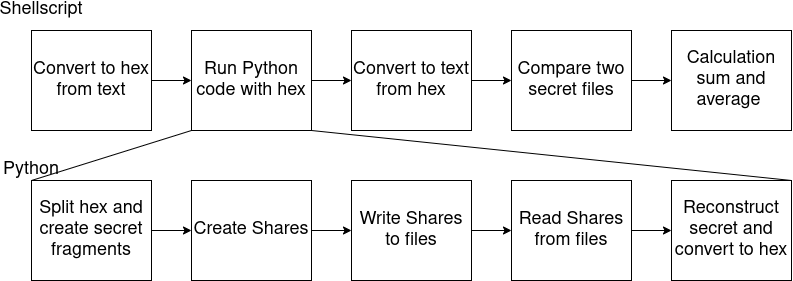
\includegraphics[scale=0.7]{program_2.png}
			\caption{実装したプログラム全体の流れ.}
			\label{program}
		\end{center}
	\end{figure}

	\section{シェルスクリプト部}
	シェルスクリプトのみの流れを示したものを図\ref{shellscript}に示す.

	まず,引数として受け取った秘密ファイルをxxdコマンドで16進数に変換し,1行あたり512ビットずつ書き込んでファイルとして保存する.
	%
	次に,16進数のファイルをPythonのプログラムに渡して実行する.
	%
	このとき,timeコマンドを用いて実行することで,実行にかかった時間を計測している.
	%
	その後,Pythonのプログラムによって生成された16進数のファイルをxxdコマンドでテキストに変換し,元のテキストファイルと再構築された秘密ファイルの差分をdiffコマンドで比較する.
	%
	最後に,Pythonによって生成された各シェアのサイズから,合計と平均を求めて表示する.

	\begin{figure}[ht]
		\begin{center}
			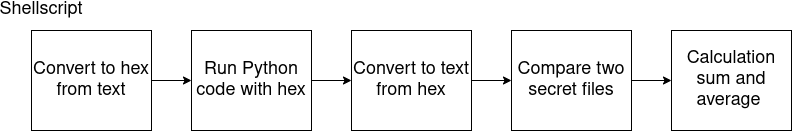
\includegraphics[scale=0.7]{shellscript_2.png}
			\caption{実装したシェルスクリプトの流れ.}
			\label{shellscript}
		\end{center}
	\end{figure}

	\section{Python部}
	Pythonのソースコードのみの流れを示したものを図\ref{python}に示す.

	ファイル入出力や秘密情報の分割については秘密分散と切り離すため別のプログラムを作成し,それぞれのアルゴリズムにインポートして使用している.

	リスト\ref{split}のファイルでは,各秘密分散には16進数を4文字ずつ読み込み,64ビット分の情報を一つの10進数の秘密情報として渡している.
	%
	リスト\ref{output}では,秘密分散によって生成されたシェアを,インデックスごとに分けてファイルに書き込んでいる.
	%

	リスト\ref{read}では,設定された数だけシェアを読み込んで,配列にしている.このとき,シェアは$1$から設定された数まで順番に利用される.
	%
	リスト\ref{reconst}では,再構築された10進数の秘密情報の配列を16進数に変換し,再構築後の16進数の秘密情報としてファイルに書き込んでいる.

	どの秘密分散においても,一つの10進数の秘密情報に対して,設定された数だけシェアを作成している.
	%
	また,今回用いている乱数のシード値は固定した.

	加法的秘密分散については,生成するシェア数を$n=11$とし,用いる乱数の範囲を$0{\leq}r{\leq}2^{16}-1$とした.
	%
	復元には$n=11$個のシェアを読み込み,単純な加算を用いた.

	$(k,n)$しきい値秘密分散では再構築可能なシェア数を$k=4$,生成するシェア数を$n=11$に設定し,有限体の標数は$p=65537$とした.
	%
	復元には$x=0$におけるラグランジュ補間を用いた.
	%
	図\ref{poly}に示すように,$x=0$において得られる関数の値は多項式の定数項とした秘密情報と一致するため,復元が可能となっている.

	\begin{figure}[ht]
		\begin{center}
			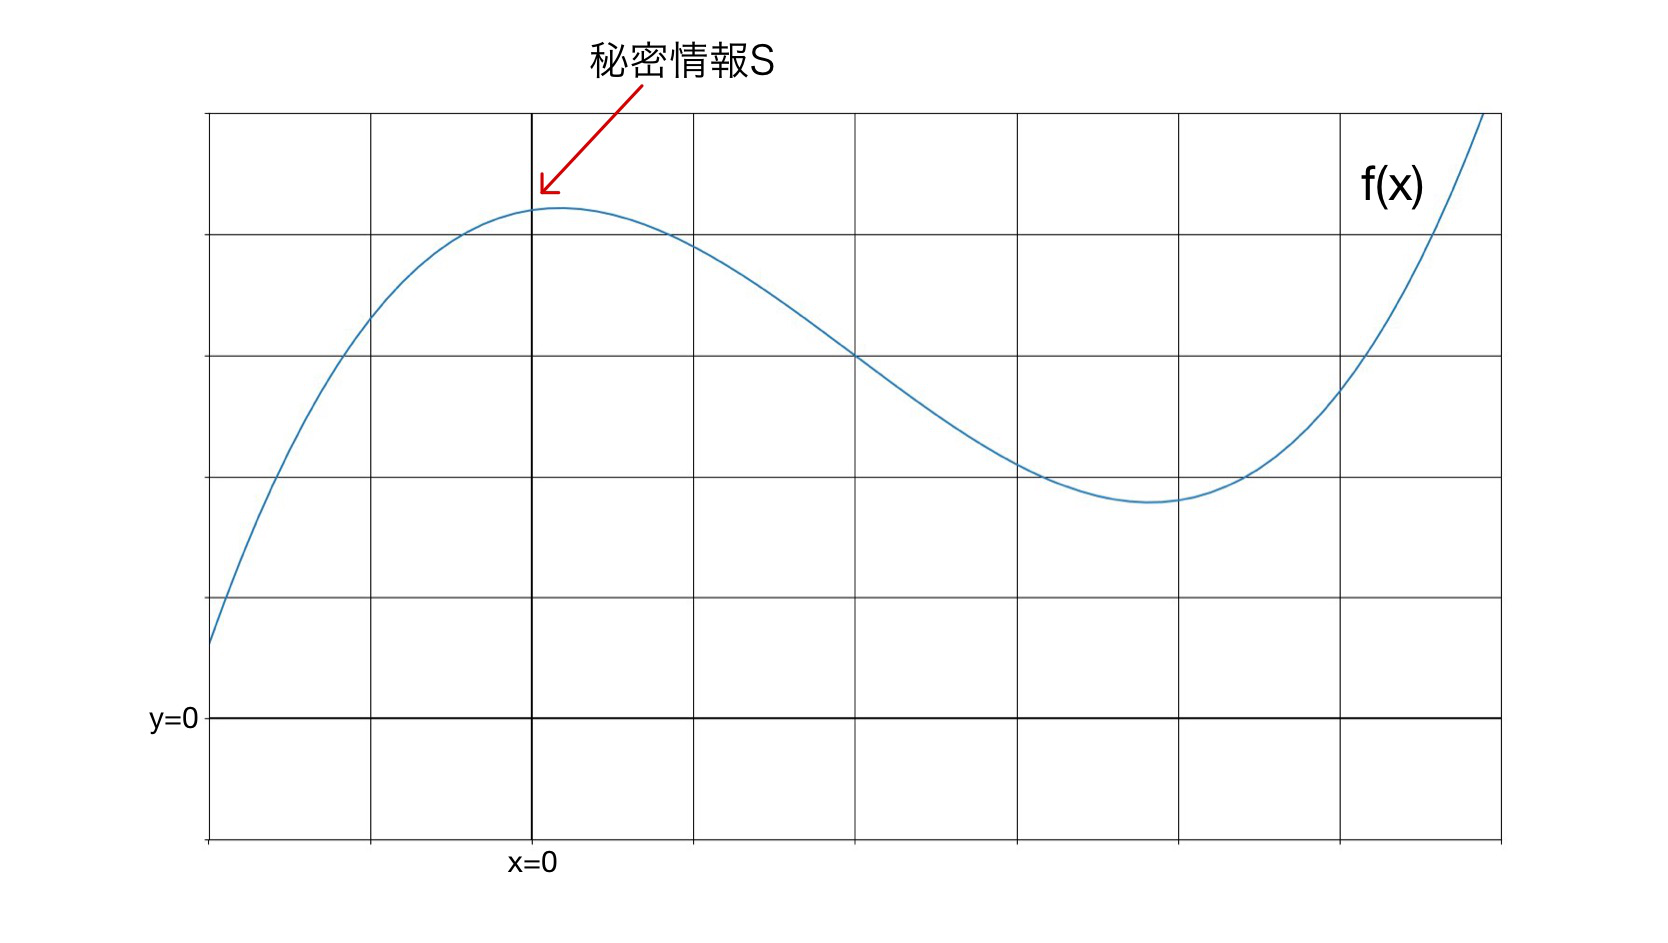
\includegraphics[scale=0.15]{poly-1.png}
			\caption{秘密情報取得の概念図.}
			\label{poly}
		\end{center}
	\end{figure}

	$(k,L,n)$しきい値秘密分散では再構築可能なシェア数を$k=4$,分割パラメータを$L=2$,生成するシェア数を$n=11$に設定し,有限体の標数は$p=65537$とした.
	%
	復元はヴァンデルモンド行列による逆行列計算を用いた.
	%
	ヴァンデルモンド行列とは,以下に示す連立方程式のうち,係数行列のような形式のものを指す.
	%
	\begin{eqnarray*}
		\left(
		\begin{array}{ccccc}
			1 & x_1 & x_1^2 & \cdots & x_1^{k-1} \\
			1 & x_2 & x_2^2 & \cdots & x_2^{k-1} \\
			1 & x_3 & x_3^2 & \cdots & x_3^{k-1} \\
			\vdots & \vdots & \vdots & \ddots & \vdots \\
			1 & x_{k-1} & x_{k-1}^2 & \cdots & x_{k-1}^{k-1} \\
		\end{array}
		\right)
		\left(
		\begin{array}{cccccccc}
			s_0 \\
			s_1 \\
			\vdots \\
			s_L \\
			a_0 \\
			a_1 \\
			\vdots \\
			a_{k-L-1}
		\end{array}
		\right)
		=
		\left(
		\begin{array}{ccccc}
			y_1 \\
			y_2 \\
			y_3 \\
			\vdots \\
			y_{k-1}
		\end{array}
		\right)
	\end{eqnarray*}

	\begin{figure}[ht]
		\begin{center}
			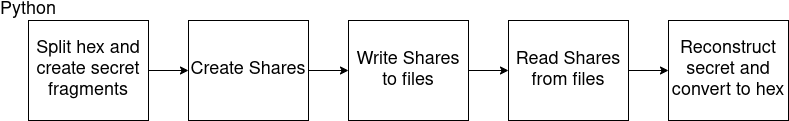
\includegraphics[scale=0.7]{python_2.png}
			\caption{実装したPythonの流れ.}
			\label{python}
		\end{center}
	\end{figure}

	\chapter{結果・考察}
	Python部のみの実行時間を計測した結果と平均シェアサイズを表\ref{table:result}に示す.
	%
	実行時間は秘密情報の分散処理及び復元処理が終わるまでの時間を示す.
	%
	また,平均シェアサイズはシェルスクリプト実行によって表示されたサイズの上位から4桁目を四捨五入した値を示す.

	\begin{table}[ht]
		\begin{center}
			\caption{実行時間及びシェアの平均サイズ.}
			\scalebox{1.1}{
			\begin{tabular}{|c|c|c|c|} \hline
				アルゴリズム & 実行時間[s] & 平均サイズ[KB] \\ \hline
				加法的秘密分散 & 2.714 & 約603 \\ \hline
				$(k,n)$しきい値秘密分散 & 6.956 & 約583 \\ \hline
				$(k,L,n)$しきい値秘密分散 & 2145.62 & 約583 \\ \hline
			\end{tabular}
			}
			\label{table:result}
		\end{center}
	\end{table}

	平均シェアサイズについては,どの秘密分散においても,最大サイズが16ビットにほぼ収まっているため大きな違いは見られなかった.
	%
	加法的秘密分散は各シェアを$0{\leq}r{\leq}2^{16}-1$の範囲でランダムに生成し,除算を行っていないため,演算を有限体上で行い,演算結果がほぼ16ビット以内になる他の二つと比べて平均シェアサイズが大きくなっている.
	%
	また今回の実装方法の場合,$(k,L,n)$しきい値秘密分散と$(k,n)$しきい値秘密分散の平均シェアサイズがほぼ同等となり,シェアサイズが$1/L$になるという性質の効果が見られなかった.
	%
	これは,$(k,L,n)$しきい値秘密分散において,一つの秘密情報を分割してから秘密分散処理を行っているためだと考えられる.
	%
	解決法として,一つの秘密情報を分割するのではなく,指定されたパラメータの分だけ秘密情報を用いて秘密分散処理を行うことがあげられる.

	実行時間について,乱数の生成や加減算のみを行うシンプルな加法的秘密分散が最も速い結果となった.
	%
	次点で$(k,n)$しきい値秘密分散が速く,$(k,L,n)$しきい値秘密分散は,今回秘密情報の断片を取り出すのに逆行列計算を用いているため非常に時間がかかった結果となった.
	%
	加法的秘密分散は復元処理に単純な加算のみを用いているため$O(n)$であり,秘密ファイルのサイズを増やしたときに実行時間は線形増加すると考えられる.
	%
	対して,$(k,n)$しきい値秘密分散は復元処理にラグランジュ補間を用いているため$O(n^{2})$,$(k,L,n)$しきい値秘密分散は復元処理に逆行列計算を用いているため$O(n^{3})$と,計算量の多い処理をしているため,非線形増加をすると考えられる.

	\chapter{まとめ}
	本研究では,加法的秘密分散・$(k,n)$しきい値秘密分散・$(k,L,n)$しきい値秘密分散及び実行やファイル入出力に関する周辺プログラムを実装し,実行速度及び生成されたシェアの容量について評価・考察した.
	%
	本研究の実装手法・評価項目においては実行時間が二番目に速く,シェアサイズが比較的小さい$(k,n)$しきい値秘密分散が最も優れているという結果となった.

	今後の展望として,まず$(k,L,n)$しきい値秘密分散について,与えられた秘密情報を再度分割するのではなく,$L$個ずつ秘密分散の処理にかけることでシェアのサイズ削減ができる.
	%
	また,逆行列計算よりも計算量の少ないアルゴリズムを検討することでより高速な動作が期待できる.
	
	加法的秘密分散に対しても,有限体上や有限環上で実装ができるため,その条件も他の2つと合わせた場合に結果にどのような影響が出るのかを比較することもあげられる.

	次に,比較対象として,AONT秘密分散\cite{rivest}やKrawczykの方式\cite{krawczyk}などを実装することで,より多くのアルゴリズムがらより良いものを選べる.
	%
	AONT(All-Or-Nothing Transform)秘密分散とは,”All-Or-Nothing form”という形式の擬似メッセージを用いた暗号を,秘密分散に応用した手法である."All-Or-Nothing form"とは,メッセージ$m_1,m_2,\cdots,m_s$に対し,以下のように計算されたメッセージ$m_i'$のことである.
	%
	\begin{eqnarray*}
		m_i'=m_i{\oplus}E(K',i) i=1,2,{\cdots},s
	\end{eqnarray*}

	ここで,$K'$は大きな空間からランダムに選んだ秘密鍵である.
	%
	上記の操作は,逆変換が可能であるため秘密分散に応用ができる.

	Krawczykの方式とは,秘密情報を暗号化し,暗号文と秘密鍵をそれぞれ別のアルゴリズムで分散処理し,分散後の情報のペアをシェアとする手法である.

	また評価項目として,一つのシェアから得られる秘密情報の情報量や,秘密の分散・再構築時にかかった時間の項目,各秘密分散について乱数の範囲やパラメータを変更した際の項目を設けたり,様々な大きさの秘密ファイルを秘密分散処理したりすることで,より多角的な評価・考察が可能となる.

	一つの情報量から得られる秘密情報の情報量を追加することで,安全性と実行時間のトレードオフについての検討などができる.
	%
	また,その他の項目追加で,秘密分散処理のどの部分に時間がかかるのかなど,詳しい性質の評価につながる.

	\begin{thebibliography}{99}
		\bibitem{shamir}
			A Shamir,
			``How to Share a Secret'',
			Communications of the ACM, Vol.22 pp612--613, 1979.

		\bibitem{oohara}
			大原一真,
			``秘密分散を用いた秘密計算'',
			システム/制御/情報, Vol.63, pp71--76, 2019.

		\bibitem{yamamoto}
			山本博資,
			``(k,L,n)しきい値秘密分散システム'',
			電子通信学会論文誌, Vol.J68-A, pp945--952, 1985.

		\bibitem{multiparty}
			千田浩司・五十嵐大・菊池亮・濱田浩気,
			``計算量的秘密分散およびランプ型秘密分散のマルチパーティ計算拡張'',
			研究報告コンピュータセキュリティ, Vol.2012-CSEC-58, pp1--5, 2012.
		\bibitem{rivest}
			Ronald L. Rivest,
			``All-or-Nothing Encryptionand the Package Transform'',
			Fast Software Encryption, Vol.LNCS 1267, pp210--218, 1997.

		\bibitem{krawczyk}
			Hugo Krawczyk,
			``Secret Sharing Made Short'',
			CRYPTO'93, Vol.LNCS 773, pp136--146, 1994.
	\end{thebibliography}

	\appendix
	\chapter{ソースコード}

	本研究で作成したソースコードを以下に示す.

	\section{シェルスクリプト部}
	結果に影響を出さないため,秘密分散のソースコード以外は同一のプログラム構造を用いている.

	今回は例として加法的秘密分散の際に用いるシェルスクリプトを示す.他2つの秘密分散では15行目のPythonファイル名,41行目のメッセージ部分を変更して利用している.
	%
	リスト\ref{.zshrc}はシェルスクリプト内で用いているtimeコマンドのフォーマットをzshの設定ファイルから一部抜粋して示している.
	%
	またリスト\ref{ASS.sh}内のtimeコマンドの引数は,ファイルパスを省略している.

	このシェルスクリプトは,実行するために対象となるファイルを用意し,引数として渡す必要がある.また,実行すると"secret.hex","secret\_reconst.hex","secret\_reconst.txt","sharesize\_sum.txt"が生成される.

	\begin{lstlisting}[caption=.zshrc(一部抜粋), label=.zshrc]
TIMEFMT=$'\n===============\nCPU	:%P\nuser	:%*Us\nsystem	:%*Ss\ntotal	:%*Es\n===============\n'
	\end{lstlisting}

	\begin{lstlisting}[caption=ASS.sh, label=ASS.sh]
#! /bin/zsh

source ~/.zshrc

if [ $# -eq 1 ]; then
	FILE1="secret.hex"
	if [ -e $1 ]; then
		xxd -p $1 > ${FILE1}
		echo "Succeeded convert to hex."
	else
		echo "Error occurred.(1)"
	fi

	if [ -e ${FILE1} ]; then
		time Python3.7 AdditiveSecretSharing.py ${FILE1}
		echo "Succeeded Secret Sharing."
	else
		echo "Error occurred.(2)"
	fi

	FILE2="secret_reconst.hex"
	FILE3="secret_reconst.txt"
	if [ -e ${FILE2} ]; then
		touch ${FILE3}
		xxd -p -r ${FILE2} > ${FILE3}
		echo "Succeeded convert to text."
	else
		echo "Error occurred.(3)"
	fi

	if [ -e ${FILE3} ]; then
		diff -s $1 ${FILE3}
		echo "Succeeded reconstruct."
	else
		echo "Error occurred.(4)"
	fi

	ls -la | grep 'Share' | cut -d ' ' -f 5 > sharesize_sum.txt
	awk '{ s += $size }; END { print "sum="s"[KB],", "average="s/NR"[KB]"}' < sharesize_sum.txt
else
	echo "usage: ./ASS.sh [file]"
fi
	\end{lstlisting}

	\section{Python部}
	Pythonでは大きく分けて2種類のソースコードを作成した.はじめに秘密分散のソースコード,次にファイル入出力関係のソースコードを示す.

	どの秘密分散においてもファイル入出力は同じファイルを用いている.

	\subsection{加法的秘密分散}

	\begin{lstlisting}[caption=AdditiveSecretSharing.py, label=ASS]
import random
import file_split as fsplit
import file_output as foutput
import file_read as fread
import file_reconst as freconst

#
# create share
#
def create_share(_secret, _n):
    share = []
    for i in range(1, _n):
        r = random.randint(0, 2**16-1)
        share.append(r)
    s = _secret - sum(share)
    share.insert(0, s)
    return share

#
# combine share
#
def combine_share(_share):
    s = sum(_share)
    return s

def main():
    #
    # define some constant
    #
    secret = fsplit.hex_to_int()
    n = 11
    random.seed(0)

    #
    # disperse imformation
    #
    shares = []
    for i in range(len(secret)):
        shares.append(create_share(secret[i], n))

    #
    # write file
    #
    temp = []
    for i in range(len(shares[0])):
        for j in range(len(shares)):
            temp.append(shares[j][i])
        foutput.write_share('Share', i + 1, temp)
        temp = []

    #
    # read file
    #
    shares = fread.read_share('Share', n)

    #
    # reconstruct imformation
    #
    re_s = []
    for i in range(len(shares)):
        s = combine_share(shares[i])
        if secret[i] == s:
            re_s.append(s)
    freconst.int_to_hex(re_s)

if __name__ == '__main__':
    main()
	\end{lstlisting}

	\subsection{$(k,n)$しきい値秘密分散}

	\begin{lstlisting}[caption=ShamirSecretSharing.py, label=SSS]
import random
import file_split as fsplit
import file_output as foutput
import file_read as fread
import file_reconst as freconst

#
# generate server ids
#
def generate_serverId(_n, _prime):
    serverId = [i + 1 for i in range(_prime - 1)]
    random.shuffle(serverId)
    for i in range(_prime -_n):
        serverId.pop(0)
    return serverId

#
# generate coefficient of polynomial
#
def generate_polynomial(_secret, _k, _prime):
    fx = [_secret]
    for i in range(_k - 1):
        fx.append(random.randint(0, _prime - 1))
    return fx

#
# create share
#
def create_share(_serverId, _fx, _prime):
    share = []
    for i in _serverId:
        temp = 0
        for j in range(len(_fx)):
            temp += _fx[j] * i ** j
        temp %= _prime
        share.append(temp)
    return share

#
# calculation of Lagrange Interpolation
#
def lagrange_interpolation(_dataX, _dataY, _prime):
    dataNum = len(_dataX)
    x = 0
    l = 0
    L = 0
    for i in range(dataNum):
        l1 = base_polynomial(dataNum, i, x, _dataX, _prime)
        l2 = base_polynomial(dataNum, i, _dataX[i], _dataX, _prime)
        temp1, l2_inv, temp2 = xgcd(l2, _prime)
        l = l1 * l2_inv
        L += _dataY[i] * l
    L %= _prime
    return L

#
# calculation of base polynomial for Lagrange Interpolation
#
def base_polynomial(_dataNum, _i, _x, _dataX, _prime):
    l = 1
    for k in range(_dataNum):
        if _i != k:
            l *= _x - _dataX[k]
    l = l % _prime
    return l

#
# calculation of inverse element on Galois Field
#
def xgcd(_a, _b):
    if _a == 0:
        return _b, 0, 1
    else:
        g, y, x = xgcd(_b%_a, _a)
        return g, x - (_b//_a)*y, y

#
# choose share randomly by the number of shareNum and make list
#
def choose_share(_serverId, _w, _n, _shareNum):
    useShare = [i for i in range(_n - 1)]
    random.shuffle(useShare)
    for i in range(_n - _shareNum):
        useShare.pop(0)
    print(f'using share number = {useShare}')
    dataX = []
    dataY = []
    for i in useShare:
        dataX.append(serverId[i - 1])
        dataY.append(w[i - 1])
    return dataX, dataY

def main():
    #
    # define some constant
    # secret:original secret  k:key num  n:share num  prime:prime
    #
    secret = fsplit.hex_to_int()
    k = 4
    n = 11
    prime = 65537
    random.seed(0)

    #
    # split secret
    # generate server id and n degree polynomial then calculate share
    #
    fx = []
    shares = []
    serverId = generate_serverId(n + 1, prime)
    for i in range(len(secret)):
        fx = generate_polynomial(secret[i], k, prime)
        shares.append(create_share(serverId, fx, prime))

    #
    # write file
    #
    for i in range(len(shares[0])):
        temp = [serverId[i]]
        for j in range(len(shares)):
            temp.append(shares[j][i])
        foutput.write_share('Share', i + 1, temp)
    
    #
    # read file
    #
    shares = fread.read_share('Share', k+1)
    dataX = []
    dataY = []
    for i in range(len(shares[0])):
        dataX.append(shares[0][i])
    for i in range(1, len(shares)):
        temp = []
        for j in range(len(shares[0])):
            temp.append(shares[i][j])
        dataY.append(temp)

    #
    # reconstruct information
    #
    re_s = []
    for i in range(len(dataY)):
        s = lagrange_interpolation(dataX, dataY[i], prime)
        if secret[i] == s:
            re_s.append(s)
    freconst.int_to_hex(re_s)

if __name__ == '__main__':
    main()
	\end{lstlisting}

	\subsection{$(k,L,n)$しきい値秘密分散}

	\begin{lstlisting}[caption=RampSecretSharing.py, label=RSS]
import random
from sympy import Matrix
import file_split as fsplit
import file_output as foutput
import file_read as fread
import file_reconst as freconst

#
# generate server ids
#
def generate_serverId(_n, _prime):
    serverId = [i+1 for i in range(_prime-1)]
    random.shuffle(serverId)
    for i in range(_prime-_n):
        serverId.pop(0)
    return serverId

#
# generate coefficient of polynomial
#
def generate_polynomial(_secret, _k, _L, _prime):
    secBit = format(_secret, 'b')
    bitLen = len(secBit)
    if bitLen%8 != 0:
        secBit = format(_secret, '0' + str(bitLen + (8 - bitLen%8)) + 'b')
        bitLen = len(secBit)
    fx = []
    for i in range(_L):
        temp = secBit[i*int(bitLen/_L):(i+1)*int(bitLen/_L)]
        fx.append(int(temp, 2))
    for i in range(_L, _k-1):
        fx.append(random.randint(0, _prime-1))
    return fx

#
# create share
#
def create_share(_serverId, _fx, _prime):
    share = []
    for i in _serverId:
        temp = 0
        for j in range(len(_fx)):
            temp += _fx[j] * i**j
        temp %= _prime
        share.append(temp)
    return share

#
# reconstruct secrets
#
def reconst_secret(_dataX, _dataY, _prime, _k, _L):
    num = len(_dataX)
    xList = []
    for x in _dataX:
        for i in range(num):
            xList.append((x ** i) % _prime)
    xMat = Matrix(num, num, xList)
    yMat = Matrix(num, 1, _dataY)
    xMat = xMat.inv_mod(_prime)
    ansMat = (xMat * yMat) % _prime

    bit = ''
    for i in range(_L):
        temp = format(int(ansMat[i]), 'b')
        if len(temp)%8 != 0:
            temp = format(int(ansMat[i]), '0' + str(len(temp) + (8 - len(temp)%8)) + 'b')
        bit += temp
    secret = int(bit, 2)
    return secret

#
# choose share randomly by the number of shareNum and make list
#
def choose_share(_serverId, _w, _n, _shareNum):
    useShare = [i for i in range(_n-1)]
    random.shuffle(useShare)
    for i in range(_n-_shareNum):
        useShare.pop(0)
    dataX = []
    dataY = []
    for i in useShare:
        dataX.append(_serverId[i-1])
        dataY.append(_w[i-1])
    return dataX, dataY

def main():
    #
    # define some constant
    # secret:original secret  k:key num  n:share num  prime:prime
    #
    secret = fsplit.hex_to_int()
    k = 4
    L = 2
    n = 11
    prime = 65537
    random.seed(0)

    #
    # split secret
    # generate server id and n degree polynomial then calculate share
    #
    fx = []
    shares = []
    serverId = generate_serverId(n+1, prime)
    for i in range(len(secret)):
        fx = generate_polynomial(secret[i], k, L, prime)
        shares.append(create_share(serverId, fx, prime))

    #
    # write file
    #
    for i in range(len(shares[0])):
        temp = [serverId[i]]
        for j in range(len(shares)):
            temp.append(shares[j][i])
        foutput.write_share('Share', i + 1, temp)

    #
    # read file
    #
    shares = fread.read_share('Share', k + 1)
    dataX = []
    dataY = []
    for i in range(len(shares[0])):
        dataX.append(shares[0][i])
    for i in range(1, len(shares)):
        temp = []
        for j in range(len(shares[0])):
            temp.append(shares[i][j])
        dataY.append(temp)
    
    #
    # reconstruct information
    #
    re_s = []
    for i in range(len(dataY)):
        s = reconst_secret(dataX, dataY[i], prime, k, L)
        if secret[i] == s:
            re_s.append(s)
    freconst.int_to_hex(re_s)

if __name__ == '__main__':
    main()
	\end{lstlisting}

	\subsection{ファイル入出力関係}
	ここでは順に「16進数の秘密ファイルを10進数の秘密情報に分割するソースコード」,「シェアをファイルに書き込むソースコード」,「シェアを指定された数だけ順に読み込むソースコード」,「再構築された10進数の秘密情報を16進数に変換するソースコード」を示す.

	\begin{lstlisting}[caption=file\_split.py, label=split]
import sys

def hex_to_int():
    if len(sys.argv) < 2:
        print('too few arguments.')
        sys.exit()
    elif len(sys.argv) > 2:
        print('too many arguments.')
        sys.exit()

    file_name = sys.argv[1]
    HEX = ''
    with open(file_name, mode='r') as s:
        for l in s:
            HEX += l
    HEX = HEX.replace('\n', '')

    size = 4
    DEC = []
    h = ''
    temp = ''
    for i in range(len(HEX)):
        h = hex(int(HEX[i], 16))
        temp += h[2:]
        if i % size == size - 1:
            DEC.append(int('0x'+temp, 16))
            temp = ''

    return DEC
	\end{lstlisting}

	\begin{lstlisting}[caption=file\_output.py, label=output]
def write_share(_name, _number, _shares):
    file_name = str(_name) + str(_number) + '.txt'
    with open(file_name, mode='w') as f:
        for i in range(len(_shares)):
            f.write(str(_shares[i])+'\n')
	\end{lstlisting}

	\begin{lstlisting}[caption=file\_read.py, label=read]
def read_share(_name, _n):
    shares = []
    for i in range(_n):
        temp = []
        filename = str(_name) + str(i + 1) + '.txt'
        with open(filename, mode='r') as f:
            for l in f:
                l = l[:-1]
                temp.append(int(l))
        shares.append(temp)
    shares = [[shares[i][j] for i in range(len(shares))] for j in range(len(shares[0]))]
    return shares
	\end{lstlisting}

	\begin{lstlisting}[caption=file\_reconst.py, label=reconst]
def int_to_hex(DEC):
    re_HEX = ''
    for i in range(len(DEC)):
        h = str(format(DEC[i], 'x'))
        re_HEX += h

    with open('secret_reconst.hex', mode='w') as f:
        f.write(re_HEX)
	\end{lstlisting}
\end{document}
